\documentclass[twoside,10pt]{article}
\usepackage{amsmath,amsfonts,amsthm,fullpage}
\usepackage{algorithm}
\usepackage{algorithmic}
\usepackage{graphicx}
\usepackage{subcaption}
\renewcommand{\qedsymbol}{\rule{0.7em}{0.7em}}

\begin{document}

\title{ISYE 6740 Homework 1}
\author{Arjun Singh}
\date{\today}
\maketitle



\section{Clustering}



Given $m$ data points $\text x^i$, $i=1,\dots, m$, $K$-means clustering algorithm groups them into $k$ clusters by minimizing the distortion function over $\{ r^{ij}, \mu^j \}$
$$J=\sum_{i=1}^m\sum_{j=1}^k r^{ij} \|\text x^i-\mu^j\|^2,$$
where $r^{ij}=1$ if $\text x^i$ belongs to the $j$-th cluster and $r^{ij}=0$ otherwise.

\begin{enumerate}

\item (10 points) Prove (using mathematical arguments) that using the squared Euclidean distance $\|\text x^i-\mu^j\|^2$ as the dissimilarity function and minimizing the distortion function, we will have 
   $$\mu^j=\frac{\sum_i r^{ij} \text x^i}{\sum_i r^{ij}}.$$
   That is, $\mu^j$ is the center of $j$-th cluster. 
   \begin{itemize}
   \item Answer:\\
   In order to minimize the distortion function $J$, we must differentiate $J$ w.r.t $\mu$ and set it equal to 0:
   \begin{proof}
   $$\frac{dJ}{d\mu} = 0$$
   We drop $\sum_{j=1}^k$ since we are looking at one cluster at a time.
   $$\implies 2\sum_{i=1}^m r^{ij} \|\text x^i-\mu^j\| = 0$$
   $$\implies 2\sum_{i=1}^m r^{ij} \text x^i = 2\sum_{i=1}^m r^{ij}\mu^j$$
   $$\implies \mu^j=\frac{\sum_i r^{ij} \text x^i}{\sum_i r^{ij}} $$
   \end{proof}
   

   \end{itemize}

\item (5 points) Prove (using mathematical arguments) that $K$-means algorithm converges to a local optimum in finite steps. 
	\begin{itemize}
   \item Answer:\\
   The cost function is a monotonically decreasing function leading to a sequence of non-increasing values that are bounded by 0.\\
   \\
   \textit{Step 1} : Assign the points to the closest center. The cost of this new cluster must be the same or lower than the previous cluster.
   $$ D (K^{i+1},\mu^{i}) \leq D(K^{i},\mu^{i})$$
   \textit{Step 2} : Re-center the cluster centers using the mean
   $$ D (K^{i+1},\mu^{i+1}) \leq D(K^{i+1},\mu^{i})$$\\
   Since we are dealing with a finite set of points, there are at maximum $K^{m}$ ways to partition $m$ points into $K$ clusters. The algorithm must converge once the cost function stop decreasing and there is no change in the cluster assignment i.e. all clusters have been visited or no point has a point closer than its current cluster center. 
   

   \end{itemize}

\item (10 points) Calculate $k$-means by hands.  Given $5$ data points configuration in Figure 1. Assume $k = 2$ and use Manhattan distance (a.k.a. the $\ell_1$ distance: given two 2-dimensional points $(x_1, y_1)$ and $(x_2, y_2)$, their distance is $|x_1 - x_2| + |y_1 - y_2|$).  Assuming the initialization of centroid as shown, after one iteration of k-means algorithm, answer the following questions. 

\begin{enumerate}
\item Show the cluster assignment;
\item Show the location of the new center;
\item Will it terminate in one step?
\end{enumerate}

\begin{figure}[h!]
\begin{center}
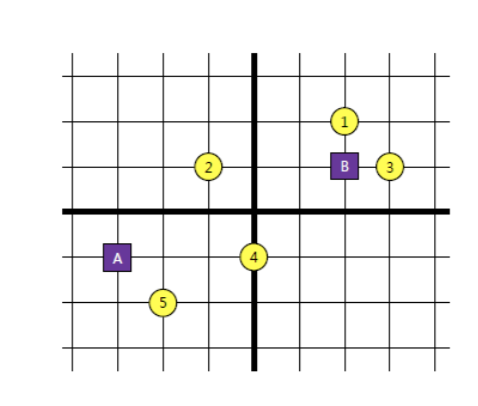
\includegraphics[totalheight=8cm]{Images/points.png}
\end{center}
\caption{K-means.}
\end{figure}

\end{enumerate}
	\begin{itemize}
   \item Answer:
   
   We can begin the k-means algorithm with the initial points. In iteration $i=1$, we assign a cluster to each data point given that $k=2$ as shown in Figure 2a. The green points correspond to cluster A and the blue points correspond to cluster B. Then we re-calculate the cluster centers A and B as shown in Figure 2b. In iteration $i=2$, we re-assign the points to the nearest cluster centers as shown in Figure 3a. Finally, re-calculate the cluster centers as shown in Figure 3b.
   
   It takes 2 iterations for the algorithm to converge, hence, it will not terminate in one step. Please refer to the attached Excel spreadhseet for the step-by-step calculations.

	
	\begin{figure*}[t!]
    \centering
    \begin{subfigure}[t]{0.5\textwidth}
        \centering
        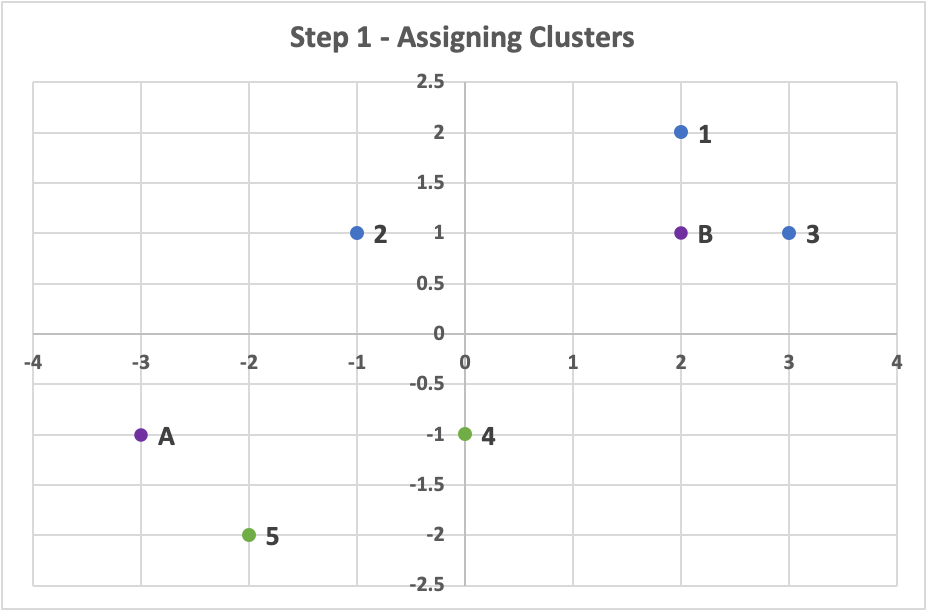
\includegraphics[height=2in]{Images/Step1.png}
        \caption{Assign Clusters to Data Points}
    \end{subfigure}%
    ~ 
    \begin{subfigure}[t]{0.5\textwidth}
        \centering
        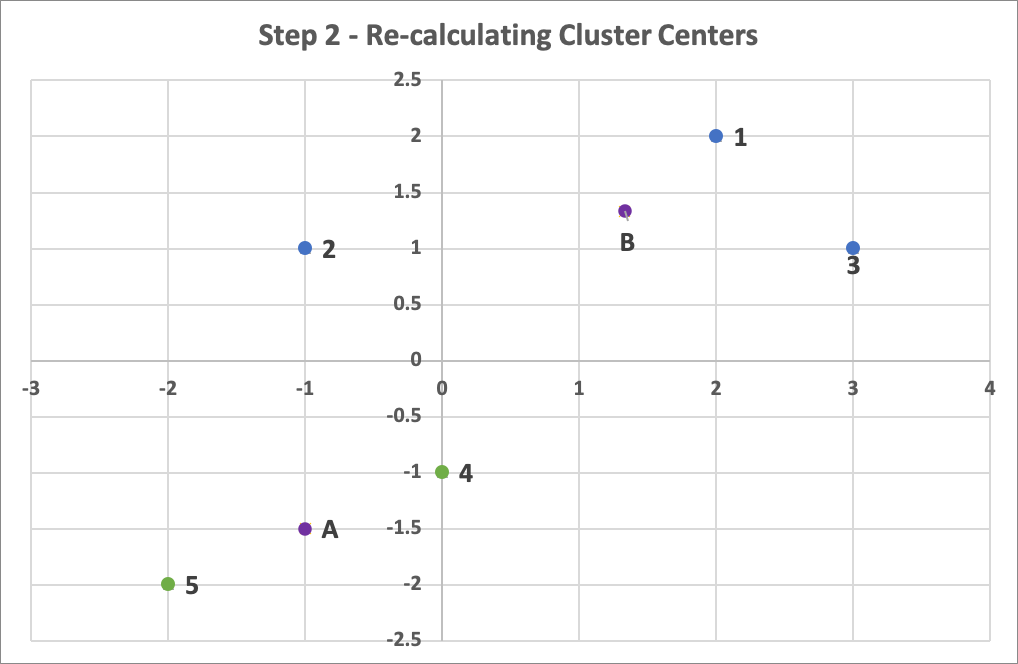
\includegraphics[height=2in]{Images/Step2.png}
        \caption{Recalculate Cluster Center}
    \end{subfigure}
    \caption{Iteration 1}
\end{figure*}

\begin{figure*}[t!]
    \centering
    \begin{subfigure}[t]{0.5\textwidth}
        \centering
        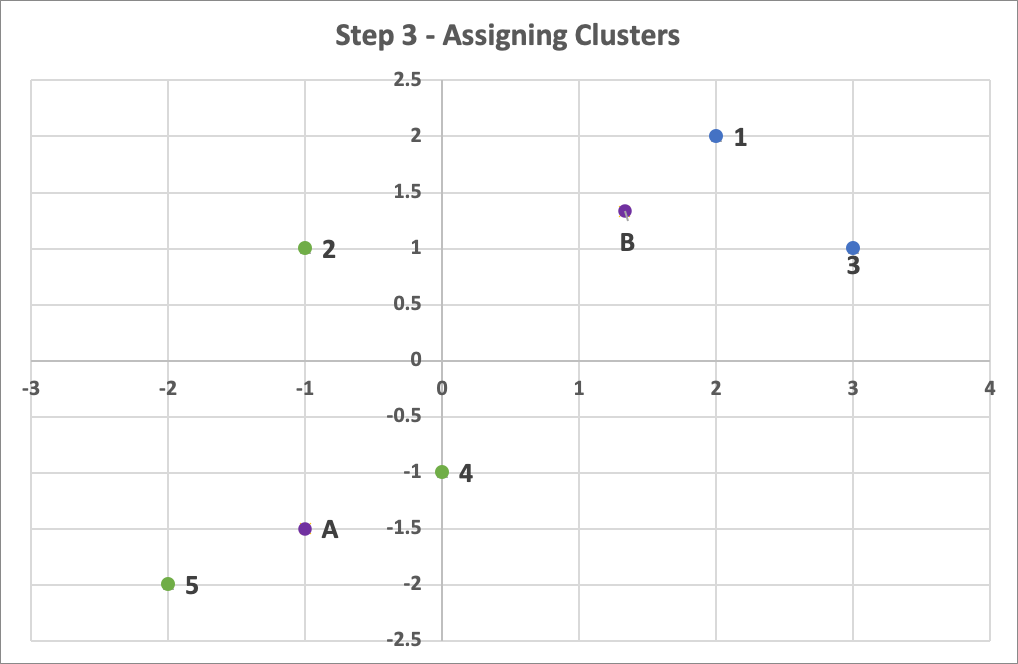
\includegraphics[height=2in]{Images/Step3.png}
        \caption{Assign Clusters to Data Points}
    \end{subfigure}%
    ~ 
    \begin{subfigure}[t]{0.5\textwidth}
        \centering
        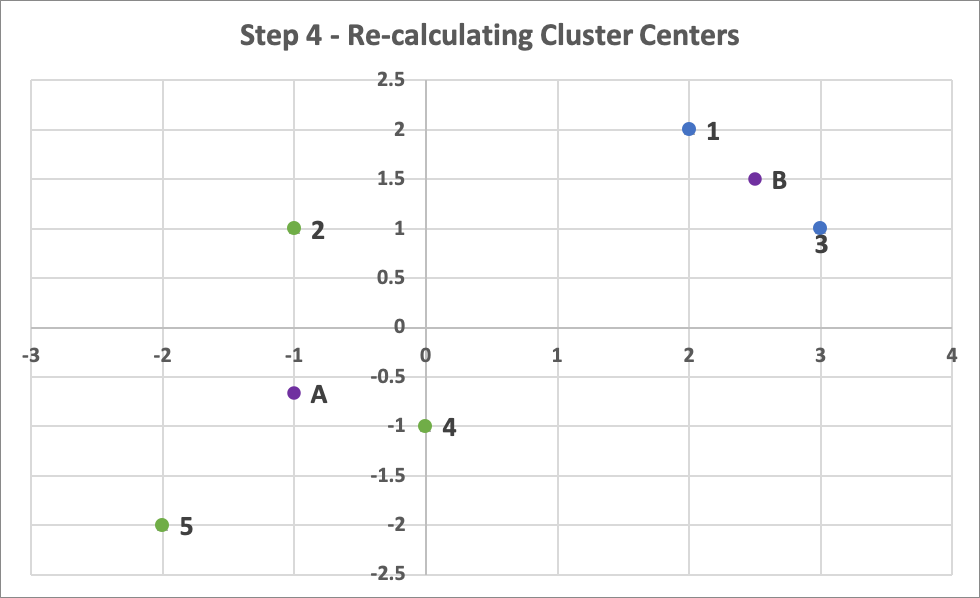
\includegraphics[height=2in]{Images/Step4.png}
        \caption{Recalculate Cluster Center}
    \end{subfigure}
    \caption{Iteration 2}
\end{figure*}



   \end{itemize}


\section{Image compression using clustering [25 points]}

In this programming assignment, you are going to apply clustering algorithms for image compression. Your task is implementing the clustering parts with two algorithms: \emph{$K$-means} and \emph{$K$-medoids}.  {\bf It is required you implementing the algorithms yourself rather than calling from a package.} %Before starting this assignment, we strongly recommend reading PRML Section 9.1.1, page 428 -- 430.

\subsubsection*{$K$-medoids}

In class, we learned that the basic $K$-means works in Euclidean space for computing distance between data points as well as for updating centroids by arithmetic mean. Sometimes, however, the dataset may work better with other distance measures. It is sometimes even impossible to compute arithmetic mean if a feature is categorical, e.g, gender or nationality of a person. With $K$-medoids, you choose a representative data point for each cluster instead of computing their average. Please note that $K$-medoid is different from generalized $K$-means: Generalized $K$-means still computes centre of a cluster is not necessarily one of the input data points (it is a point that minimizes the overall distance to all points in a cluster in a chosen distance metric). 

Given $m$ data points $\text x^i (i = 1, \ldots, m)$, $K$-medoids clustering algorithm groups them into $K$ clusters by minimizing the distortion function $J = \sum_{i=1}^m \sum_{j=1}^k r^{ij} D(\text x^i, \mu^j)$,
where $D(\text x, \text y)$ is a distance measure between two vectors $\text x$ and $\text y$ in same size (in case of $K$-means, $D(x, y) = \| \text x - \text y \|^2$), $\mu^j$ is the center of $j$-th cluster; and $r^{ij} = 1$ if $\text x^n$ belongs to the $k$-th cluster and $r^{ij} = 0$ otherwise. In this exercise, we will use the following iterative procedure:

\begin{itemize}
  \item Initialize the cluster center $\mu^j$, $j = 1, ..., k$.
  \item Iterate until convergence:
  \begin{itemize}
    \item Update the cluster assignments for every data point $\text x^i$: $r^{ij} = 1$ if $j = \arg\min_j D(\text x^i, \mu^j)$, and $r^{ij} = 0$ otherwise.
    \item Update the center for each cluster $j$: choosing another representative if necessary.
  \end{itemize}
\end{itemize}

There can be many options to implement the procedure; for example, you can try many distance measures in addition to Euclidean distance, and also you can be creative for deciding a better representative of each cluster. We will not restrict these choices in this assignment. You are encouraged to try many distance measures as well as way of choosing representatives (e.g., $\ell_1$ norm).

\subsubsection*{Formatting instruction}


\textbf{Input}
\begin{itemize}
  \item \texttt{pixels}: the input image representation. Each row contains one data point (pixel). For image dataset, it contains 3 columns, each column corresponding to Red, Green, and Blue component. Each component has an integer value between 0 and 255.
  \item \texttt{k}: the number of desired clusters. Too high value of $K$ may result in empty cluster error. Then, you need to reduce it.
\end{itemize}

\textbf{Output}
\begin{itemize}
  \item \texttt{class}: cluster assignment of each data point in pixels. The assignment should be 1, 2, 3, etc. For $k = 5$, for example, each cell of class should be either 1, 2, 3, 4, or 5. The output should be a column vector with \texttt{size(pixels, 1)} elements.
  \item \texttt{centroid}: location of $k$ centroids (or representatives) in your result. With images, each centroid corresponds to the representative color of each cluster. The output should be a matrix with $K$ rows and 3 columns. The range of values should be [0, 255], possibly floating point numbers.
\end{itemize}

\subsubsection*{Hand-in}
Both of your code and report will be evaluated. Upload them together as a zip file. In your report, answer to the following questions:
\begin{enumerate}
  \item (5 points) Within the $k$-medoids framework, you have several choices for detailed implementation. Explain how you designed and implemented details of your $K$-medoids algorithm, including (but not limited to) how you chose representatives of each cluster, what distance measures you tried and chose one, or when you stopped iteration.
  \begin{itemize}
  \item Answer:
  
  For my implementation of the k-medoids algorithm, I began by choosing randomly assigned cluster centers from the given dataset (image). I used the L1 and L2 norms to calculate the distances between the points in order to understand the effect of the distance measure on the overall efficiency of the algorithm.
  
  I chose the representatives for each cluster by first assigning the cluster labels to each data point. Then, in order to increase the efficiency of the algorithm while calculating distances, I removed any duplicate data points. From there, I calculated the distance from each point to every other point within each cluster and assigned the cluster center to the point that had the least distance to all other points.
  
  For the stopping criteria, I mulled around with a few different approaches. In the end, I decided to terminate the algorithm when the Within-Cluster-Sum-of-Squares errors decreased by less than 5\% over the previous iteration. Also, if k was too large (i.e. leading to empty clusters), I reset the value of k to an acceptable limit.
  
  \end{itemize}
  
  \item (10 points) Attach a picture of your own. We recommend size of $320 \times 240$ or smaller. Run your $k$-medoids implementation with the picture you chose, as well as two pictures provided (\textsf{beach.bmp} and \textsf{football.bmp}), with several different $K$. (e.g, small values like 2 or 3, large values like 16 or 32) What did you observe with different $K$? How long does it take to converge for each $K$? Please write in your report.
  
  \begin{itemize}
  \item Answer:\\
  For this part of the question, I decided to use an image of Tech Tower$^1$ along with the 2 images provided in the homework package. My observations were the following:
  \begin{itemize}
  \item Smaller values of k lead to a more "washed-out" images with fewer colors. This is expected since the number of clusters dictate how well the image is partitioned and how many colors show on the image. Smaller values of k also led to longer runtimes of the algorithm. This was due to the fact that there are more points within each cluster and hence, there are more computations(i.e. swaps) that need to be performed in order to find the new cluster center in each iteration. On the contrary, higher values of k produced much clearer images with more color while also running much more quickly as compared to smaller values of k. The results from the k-medoids algorithm can be seen in Figures 4, 5 and 6 as well as the attached code.
  
  
\begin{figure}
\begin{subfigure}{.5\textwidth}
  \centering
  % include first image
  
\includegraphics[height=1.5in]{Images/TechTower.jpg}  
  \caption{Original Image}
  \label{fig:sub-first}
\end{subfigure}
\begin{subfigure}{.5\textwidth}
  \centering
  % include second image
  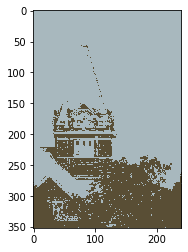
\includegraphics[height=1.5in]{Images/TechTowerKMedoids2.png}  
  \caption{K = 2, Runtime = 63.29 Seconds}
  \label{fig:sub-second}
\end{subfigure}

\begin{subfigure}{.5\textwidth}
  \centering
  % include third image
  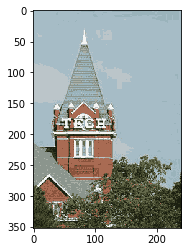
\includegraphics[height=1.5in]{Images/TechTowerKMedoids12.png}  
  \caption{K = 12, Runtime = 29.06 Seconds}
  \label{fig:sub-third}
\end{subfigure}
\begin{subfigure}{.5\textwidth}
  \centering
  % include fourth image
  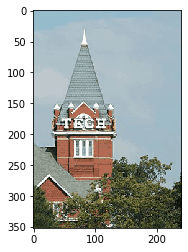
\includegraphics[height=1.5in]{Images/TechTowerKMedoids100.png}  
  \caption{K = 100, Runtime = 25.00 Seconds}
  \label{fig:sub-fourth}
\end{subfigure}
\caption{K-Medoids on Tech Tower}
\label{fig:fig}
\end{figure}  

\begin{figure}
\begin{subfigure}{.5\textwidth}
  \centering
  % include first image
  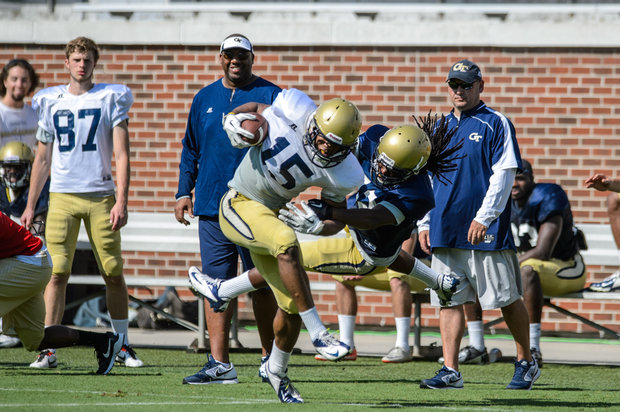
\includegraphics[height=1.5in]{Images/football.png}  
  \caption{Original Image}
  \label{fig:sub-first}
\end{subfigure}
\begin{subfigure}{.5\textwidth}
  \centering
  % include second image
  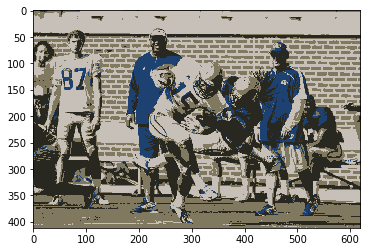
\includegraphics[height=1.5in]{Images/footballkmedoids4.png}  
  \caption{K = 4, Runtime = 380.82 Seconds}
  \label{fig:sub-second}
\end{subfigure}

\begin{subfigure}{.5\textwidth}
  \centering
  % include third image
  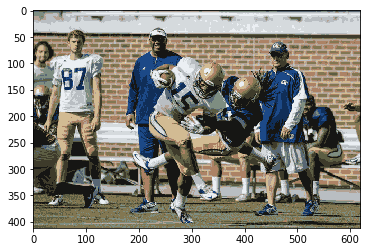
\includegraphics[height=1.5in]{Images/footballkmedoids14.png}  
  \caption{K = 14, Runtime = 153.89 Seconds}
  \label{fig:sub-third}
\end{subfigure}
\begin{subfigure}{.5\textwidth}
  \centering
  % include fourth image
  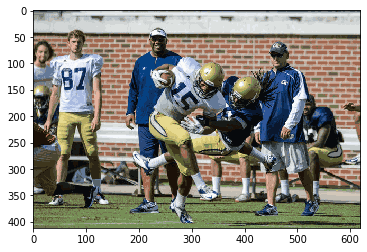
\includegraphics[height=1.5in]{Images/footballkmedoids50.png}  
  \caption{K = 50, Runtime = 130.47 Seconds}
  \label{fig:sub-fourth}
\end{subfigure}
\caption{K-Medoids on Football}
\label{fig:fig}
\end{figure}  

\begin{figure}
\begin{subfigure}{.5\textwidth}
  \centering
  % include first image
  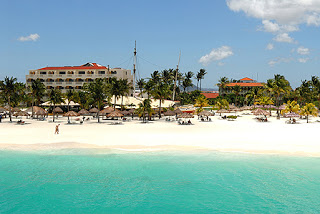
\includegraphics[height=1.5in]{Images/beach.png}  
  \caption{Original Image}
  \label{fig:sub-first}
\end{subfigure}
\begin{subfigure}{.5\textwidth}
  \centering
  % include second image
  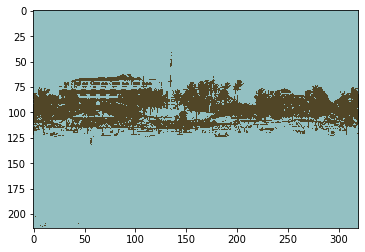
\includegraphics[height=1.5in]{Images/beachkmedoids2.png}  
  \caption{K = 2, Runtime = 64.38 Seconds}
  \label{fig:sub-second}
\end{subfigure}

\begin{subfigure}{.5\textwidth}
  \centering
  % include third image
  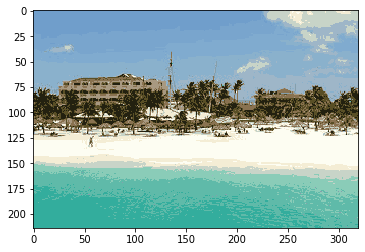
\includegraphics[height=1.5in]{Images/beachkmedoids16.png}  
  \caption{K = 16, Runtime = 25.94 Seconds}
  \label{fig:sub-third}
\end{subfigure}
\begin{subfigure}{.5\textwidth}
  \centering
  % include fourth image
  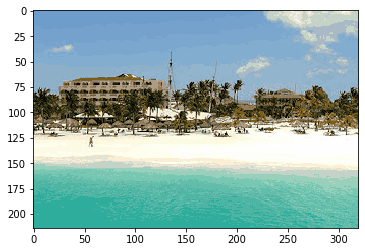
\includegraphics[height=1.5in]{Images/beachkmedoids32.png}  
  \caption{K = 32, Runtime = 37.14 Seconds}
  \label{fig:sub-fourth}
\end{subfigure}


\caption{K-Medoids on Beach}
\label{fig:fig}
\end{figure}  
  
  
  \end{itemize}
  
  $^1$J. Glover (AUtiger) / CC BY-SA (https://creativecommons.org/licenses/by-sa/2.5)
\end{itemize}   
  \item (5 points) Run your $k$-medoids implementation with different initial centroids/representatives. Does it affect final result? Do you see same or different result for each trial with different initial assignments? (We usually randomize initial location of centroids in general. To answer this question, an intentional poor assignment may be useful.) Please write in your report. 
  
  \begin{itemize}
  \item Answer\\
  To answer this part of the question, I decided to first use the same initialization points for all the clusters (instead of a randomized approach). This led to some poor results with the algorithm not being able to separate the clusters quickly and hitting the termination criteria fairly early. The algorithm also took longer than its randomized counterpart. Figure 7a shows an example of the results with K=100 with all initial clusters assigned to the same point.
  
  For another example, I tried using different randomized points as initial points to see the effect on the outcome. For lower values of k, such as k=2, there were some differences in the output image. In Figure 7b-d, we see that the same image of the beach had differing outputs. This is expected since the initial cluster assignment dictates how the image and the colors are segregated. With higher values of k, this problem disappears as there are many clusters leading to a similar output each time.
  
  \begin{figure}
\begin{subfigure}{.5\textwidth}
  \centering
  % include first image
  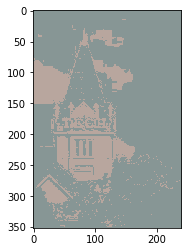
\includegraphics[height=1.5in]{Images/TechTowerSameInitPoints.png}  
  \caption{K=100, Runtime = 55.11 seconds}
  \label{fig:sub-first}
\end{subfigure}
\begin{subfigure}{.5\textwidth}
  \centering
  % include second image
  \includegraphics[height=1.5in]{Images/Beachkmedoids2.png}  
  \caption{K = 2, Runtime = 64.38 Seconds}
  \label{fig:sub-second}
\end{subfigure}

\begin{subfigure}{.5\textwidth}
  \centering
  % include third image
  \includegraphics[height=1.5in]{Images/Beachkmedoids2Run2.png}  
  \caption{K = 2, Runtime = 71.01 Seconds}
  \label{fig:sub-third}
\end{subfigure}
\begin{subfigure}{.5\textwidth}
  \centering
  % include fourth image
  \includegraphics[height=1.5in]{Images/Beachkmedoids2Run3.png}  
  \caption{K = 2, Runtime = 85.63 Seconds}
  \label{fig:sub-fourth}
\end{subfigure}
\caption{K-medoids with altered initial points}
\label{fig:fig}
\end{figure}  

  \end{itemize}
  \item (5 points) Repeat question 2 and 3 with $k$-means. Do you see significant difference between $K$-medoids and $k$-means, in terms of output quality, robustness, or running time? Please write in your report. 
  
  \begin{itemize}
  \item Answer:\\
  For my k-means algorithm, I decided to use as stopping criteria where the algorithm stops if the new cluster centers are the same as the old cluster centers. Figure 8, 9 and 10 shows the results from the k-means algorithm. In general, my observations were:
  \begin{itemize}
  \item K-means tended to produce better, sharper images. I can attribute this to the fact that the k-means algorithm uses the average of all points within a cluster rather than a point from within the cluster. This can help it make better segments and produce a sharper image.
  \item K-means was also slightly faster in my test cases. Again, this is probably due to the fact that the algorithm simply computes the average of all data points rather than calculating distances between each point like the k-medoids algorithm, leading to better runtimes (in the final images shown in the figures, my k-means algorithm takes longer, however, this is due to the fact that I have changed the stopping criteria and the k-means algorithm only stops when it converges completely).
  \item The k-means fails when all the initial centers are the same point. I tried initializing the centers to be the same point in order to test the output, however, the resulting image was a solid color. This is due to the fact that k-means assigns labels based on the closest center and since all points have the same center, they will be assigned the same label. This leads to empty clusters. This differs from k-medoids as k-medoids only chooses a new center based on the existing points rather than computing an average. This helps ensure that the algorithm has a way of continuing and partitioning the points rather than converging in 1 step.
  \item The k-means algorithm gave similar results when different initial centers were chosen. 
  \end{itemize}
  
  
  \begin{figure}
    \begin{subfigure}{.5\textwidth}
  \centering
  % include first image
  
\includegraphics[height=1.5in]{Images/TechTower.jpg}  
  \caption{Original Image}
  \label{fig:sub-first}
\end{subfigure}
\begin{subfigure}{.5\textwidth}
  \centering
  % include first image
  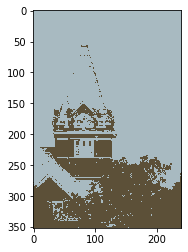
\includegraphics[height=1.5in]{Images/techtowerkmeans2.png}  
  \caption{K = 2, Runtime = 18.93 seconds}
  \label{fig:sub-first}
\end{subfigure}
\begin{subfigure}{.5\textwidth}
  \centering
  % include second image
  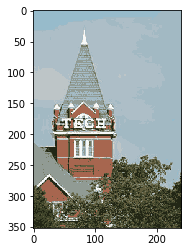
\includegraphics[height=1.5in]{Images/techtowerkmeans12.png}  
  \caption{K = 12, Runtime = 238.52 Seconds}
  \label{fig:sub-second}
\end{subfigure}
\begin{subfigure}{.5\textwidth}
  \centering
  % include second image
  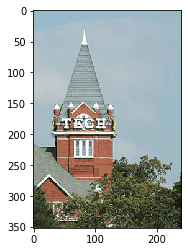
\includegraphics[height=1.5in]{Images/techtowerkmeans50.png}  
  \caption{K = 50, Runtime = 721.04 Seconds}
  \label{fig:sub-third}
\end{subfigure}

\caption{K-means on Tech Tower}
\label{fig:fig}
\end{figure}  
  
\begin{figure}
    \begin{subfigure}{.5\textwidth}
  \centering
  % include first image
  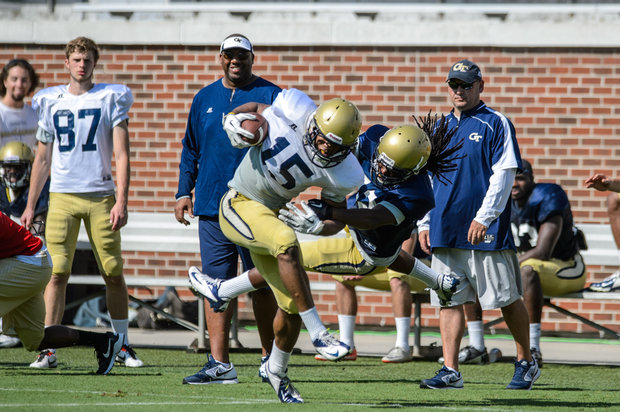
\includegraphics[height=1.5in]{Images/football.png}  
  \caption{Original Image}
  \label{fig:sub-first}
\end{subfigure}
\begin{subfigure}{.5\textwidth}
  \centering
  % include first image
  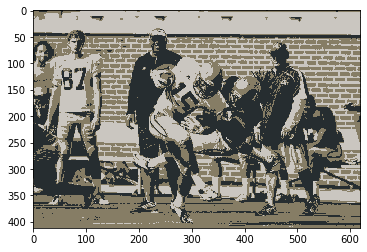
\includegraphics[height=1.5in]{Images/footballkmeans3.png}  
  \caption{K = 3, Runtime = 133.51 seconds}
  \label{fig:sub-first}
\end{subfigure}
\begin{subfigure}{.5\textwidth}
  \centering
  % include second image
  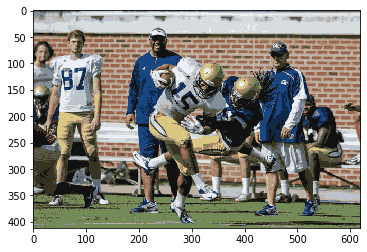
\includegraphics[height=1.5in]{Images/footballkmeans16.png}  
  \caption{K = 16, Runtime = 977.91 Seconds}
  \label{fig:sub-second}
\end{subfigure}
\begin{subfigure}{.5\textwidth}
  \centering
  % include second image
  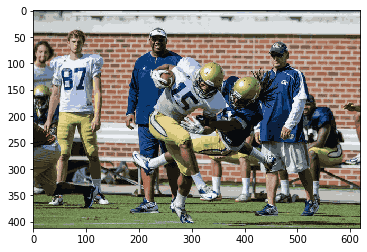
\includegraphics[height=1.5in]{Images/footballkmeans32.png}  
  \caption{K = 32, Runtime = 1025.84 Seconds}
  \label{fig:sub-third}
\end{subfigure}

\caption{K-means on Football}
\label{fig:fig}
\end{figure}   
  
  
  
    \begin{figure}
    \begin{subfigure}{.5\textwidth}
  \centering
  % include first image
  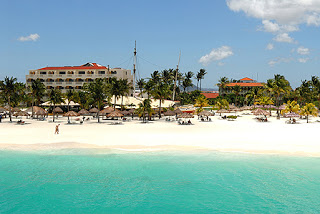
\includegraphics[height=1.5in]{Images/beach.png}  
  \caption{Original Image}
  \label{fig:sub-first}
\end{subfigure}
\begin{subfigure}{.5\textwidth}
  \centering
  % include first image
  \includegraphics[height=1.5in]{Images/Beachkmeans2.png}  
  \caption{K = 2, Runtime = 21.04 seconds}
  \label{fig:sub-first}
\end{subfigure}
\begin{subfigure}{.5\textwidth}
  \centering
  % include second image
  \includegraphics[height=1.5in]{Images/Beachkmeans16.png}  
  \caption{K = 16, Runtime = 25.94 Seconds}
  \label{fig:sub-second}
\end{subfigure}
\begin{subfigure}{.5\textwidth}
  \centering
  % include second image
  \includegraphics[height=1.5in]{Images/Beachkmeans32.png}  
  \caption{K = 32, Runtime = 412.81 Seconds}
  \label{fig:sub-third}
\end{subfigure}

\caption{K-means on Beach}
\label{fig:fig}
\end{figure}  
  
  
  
  \end{itemize}
\end{enumerate}


\subsubsection*{Note}
\begin{itemize}
  \item You may see some error message about empty clusters when you use too large $k$. Your implementation should treat this exception as well. That is, do not terminate even if you have an empty cluster, but use smaller number of clusters in that case.

  \item We will grade using test pictures which are not provided. We recommend you to test your code with several different pictures so that you can detect some problems that might happen occasionally. 

  \item If we detect copy from any other student's code or from the web, you will not be eligible for any credit for the entire homework, not just for the programming part. Also, directly calling built-in functions or from other package functions is not allowed.
\end{itemize}


\section{Spectral clustering [25 points]}


\begin{enumerate}

\item (10 points) For the following data (two moons), give one method that will successfully separate the two moons? Explain your rationale. 
\begin{itemize}
\item Answer:\\
The two moons image can be separated using spectral clustering. Since this image consists of 2 distinct geometries, an algorithm such as k-means would be inadequate as it would be unable to discern the 2 shapes. It would simply calculate the centers in Euclidean space and assign cluster labels based on on the distances to the centers. 

In order to correctly separate the two shapes, we would first need to build the adjacency matrix. In this case, we can use a similarity measure where two points are similar if we can reach them through small jumps (i.e. closely connected points will be grouped together such as the points in each half of the moon). Then we form the Laplacian matrix and compute the k eigenvectors of L. Once we have the eigenvectors, we can run k-means on this matrix formed by the eigenvectors to find the appropriate clusters.

\end{itemize}

\begin{center}
\end{center}



\item (15 points) Political blogs dataset. 

We will study a political blogs dataset first compiled for the paper Lada A. Adamic and Natalie Glance, ``The political blogosphere and the 2004 US Election'', in Proceedings of the WWW-2005 Workshop on the Weblogging Ecosystem (2005). The dataset \textsf{nodes.txt} contains a graph with $n = 1490$ vertices (``nodes'') corresponding to political blogs. Each vertex has a 0-1 label (in the 3rd column) corresponding to the political orientation of that blog. We will consider this as the true label and try to reconstruct the true label from the graph using the spectral clustering on the graph. The dataset \textsf{edges.txt} contains edges between the vertices. You may remove isolated nodes (nodes that are not connected any other nodes). 


\begin{enumerate}
\item (10 points)  Assume the number of clusters to be estimated is $k = 2$. Using spectral clustering to find the 2 clusters. Compare the clustering results with the true labels. What is the false classification rate (the percentage of nodes that are classified incorrectly). {\bf It is required you implementing the algorithms yourself rather than calling from a package.}
\begin{itemize}
\item Answer:\\
To begin this problem, I visualized the given data as shown in Figure 11. As seen in the graph, there are some outliers in the data as well as some null values. In order to proceed, I first cleaned the data by removing such points. Then, based on the edge list, I separated the graph based on the political orientation of the blog.

After running the spectral clustering algorithm, the accuracy of the algorithm was 42.73\% (i.e. the false classification rate was 57.27\%).
\begin{figure}
\centering
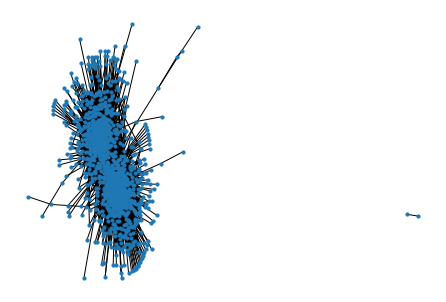
\includegraphics[height=2in]{Images/InitialCluster.png}
\caption{Original Cluster from Dataset}
\end{figure}
\end{itemize}

\item (5 points) You might observe the performance is not as good as you expected (given that there is no coding bugs). What do you think might be the reason for the not-so-good performance, due to the discrepancy from ``theory'' and ``application''? Please write in your report. 
\begin{itemize}
\item Based on theory, the spectral clustering algorithm is supposed to help identify clusters within a graph. As demonstrated in class, an example of such use would be identifying clusters of interests (such as sports, games etc.) in a social network graph.
In this problem, we have a graph of political blogs that are separated only by their political orientation, which is binary (0 or 1). As seen in Figure 12, the original graph is very tightly inter-connected with no discernible communities. Hence, when we run the spectral clustering algorithm, we get a very high false classification rate ($\geq$ 50\%).
In order to obtain a higher accuracy, we can potentially add more factors into the dataset. Apart from political orientation, if we had more details about the blogs such as geography, author, gender, amount of page visits etc., we could adjust our similarity criteria. This way, we would be better able to identify clusters based on a number of different factors rather than just the political orientation.

\end{itemize}
\end{enumerate}

\end{enumerate}

 \begin{figure}
    \begin{subfigure}{.5\textwidth}
  \centering
  % include first image
  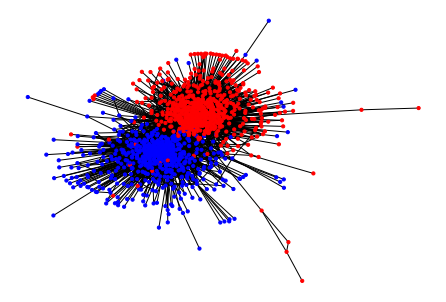
\includegraphics[height=2in]{Images/InitialClusterCleaned.png}  
  \caption{Original Cluster - Cleaned}
  \label{fig:sub-first}
\end{subfigure}
\begin{subfigure}{.5\textwidth}
  \centering
  % include first image
  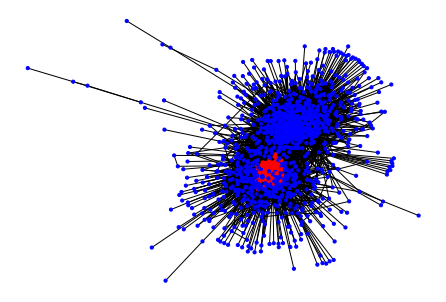
\includegraphics[height=2in]{Images/PredictedCluster.png}  
  \caption{Predicted Cluster}
  \label{fig:sub-first}
\end{subfigure}


\caption{Spectral Clustering}
\label{fig:fig}
\end{figure}

\section{PCA: Food consumption in European area [25 points]}

The data \textsf{food-consumption.csv} contains 16 countries in the European area and their consumption for 20 food items, such as tea, jam, coffee, yoghurt, and others. There are some missing data entries: you may remove the rows ``Sweden", ``Finland", and ``Spain''. The goal is to perform PCA analysis on the data, i.e., find a way to perform linear combinations of features across all 20 food-item consumptions, for each country. If we extract two principal components, that means we use two singular vectors that correspond to the largest singular values of the data matrix, in combining features. 
\begin{enumerate}
\item (5 points) Write down the set-up of PCA for this setting. Explain how the data matrix is set-up in this case (e.g., each dimension of the matrix correspond to what.) Explain in words how PCA is performed in this setting.
\begin{itemize}

\item Answer:\\
To begin this problem, we first want to perform some data cleaning. We remove all the data points that are null. The goal of PCA is to help reduce the dimensionality of the input data in order to extract the most important variables while also keeping them independent. In this case, we have 20 variables that correspond to the intake of various foods and are related to 13 countries. We want to reduce these 20 variables to 2 vectors that give us the most amount of information (i.e. capture the highest variability in the data).

The first step of PCA in this scenario is to normalize the data points. This is done due to the fact that each of the variables are on different scales and need to be standardized before running PCA. Then, we take the mean of each of the variables and estimate the covariance matrix from the dataset. Then, we find the corresponding eigenvalues and eigenvectors of the covariance matrix to construct the principal components.

\end{itemize} 
\item (5 points) Suppose we aim to find top $k$ principal components. Write down the mathematical optimization problem involved for solving this problem. Explain the procedure to find the top $k$ principal components in performing PCA. 
\begin{itemize}
\item Answer:\\
In order to perform PCA, we want to find direction $w$ where $\|w\| \leq 1$ such that the variance along the direction $w$ is maximized.
The optimization problem for PCA is the following:
$$max_{w:\|w\|\leq 1} w^TCw$$
where $w$ corresponds to the eigenvectors and $C$ to the covariance matrix.
If the covariance matrix is symmentric, this turns into an eignevalue problem. We can find $w$ such that 
$$Cw = \lambda w$$
From this, the variance in the principal direction can be explained by $\lambda$

$$w^{T}Cw = \lambda w^{T}w$$
If the covariance matrix is not symmetric, we can decompose the covariance matrix using singular value decomposition in order to find the eigenvectors. The top k principal components correspond to the k eigenvectors after performing PCA.

\end{itemize}

\item (7 points) Find the top two {\bf principal direction vectors (i.e., the eigenvectors of $C$)} for the dataset and plot them (plot a value of the vector as a one-dimensional function). Describe do you see any pattern. You may either use a package or write your own code. 
\begin{itemize}
\item Answer:\\
Using the PCA package from the sklearn library, I performed PCA on the cleaned dataset. From this I obtained 2 principal components shown in Figure 13. For principal component 1, it can be noted that the highest magnitude occurs at 'Tinned Fruit' and 'Sweetener' at around -0.3. Similarly, the highest magnitudes for principal component 2 occur at -0.4 with 'Real Coffee' and 'Frozen Fish'. Hence, these particular food items account for a high degree of variance. It can also be noted that for principal component 1, olive oil and garlic are positive while the other food items are negative. This suggests that olive Oil and Garlic tend to pair together (which is true in some cases such as Italian dishes).

From further analysis, principal component 1 accounts for 33.58\% of the variance whereas principal component 2 accounts for 16.71\% of the variance. The cumulative variance for the 2 principal components is 50.3\%.

Figure 14 shows the food items plotted with the  principal component axes. This allows us to see a better grouping of the items based on the top 2 principal components that we found. We see that items such as olive oil and garlic are grouped together, which is common in Mediterranean cooking. We also see items such as Tea, Biscuits, Jam and Instant Coffee grouped together, which is expected due to these items being common breakfast staples in European countries.

\end{itemize}

\begin{figure}
    \begin{subfigure}{.8\textwidth}
  \centering
  % include first image
  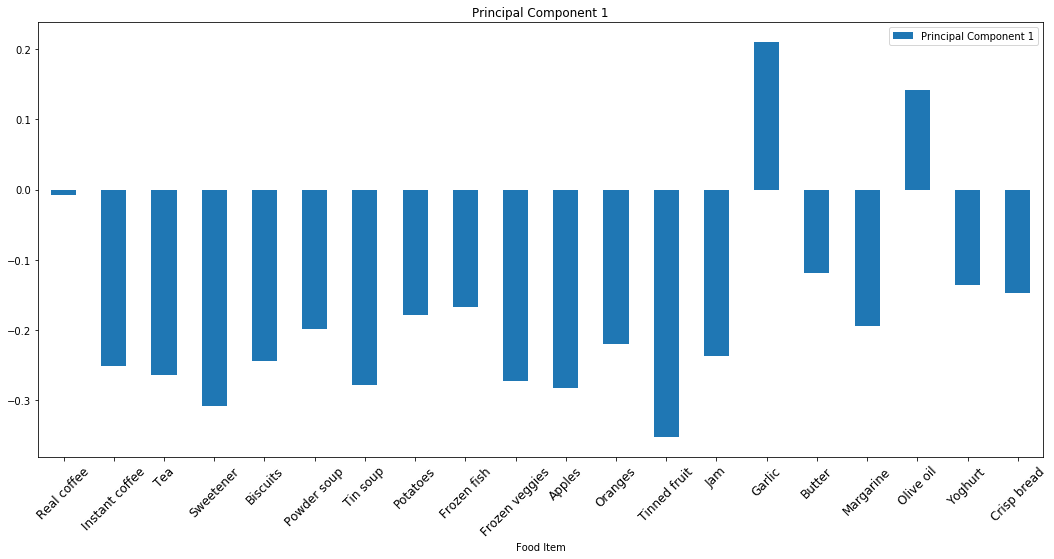
\includegraphics[height=2.5in]{Images/PCA1.png}  
  \caption{Principal Component 1}
  \label{fig:sub-first}
\end{subfigure}
\centering
\begin{subfigure}{.8\textwidth}
  \centering
  % include first image
  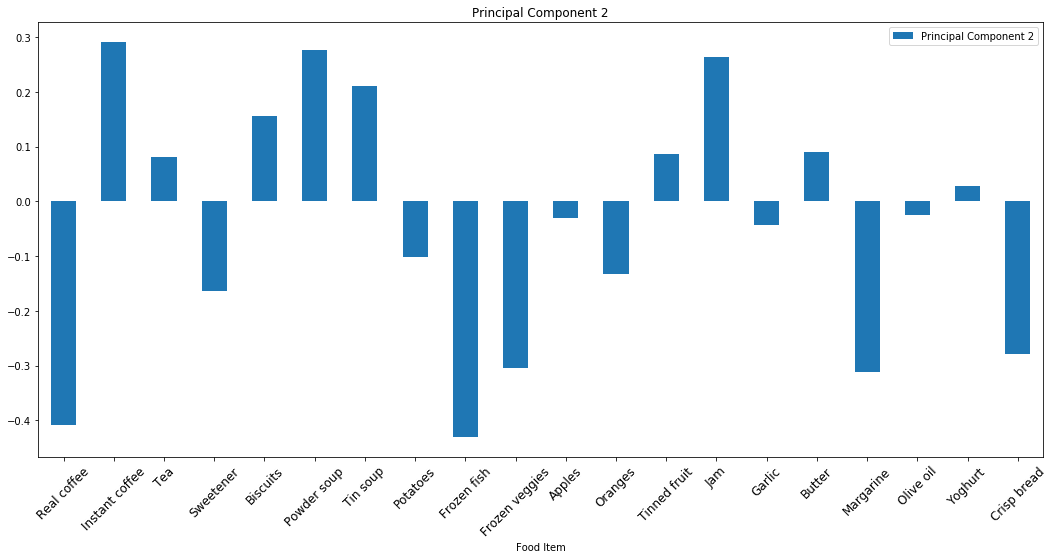
\includegraphics[height=2.5in]{Images/PCA2.png}  
  \caption{Principal Component 2}
  \label{fig:sub-first}
\end{subfigure}
\caption{Principal Component Analysis}
\label{fig:fig}
\end{figure}

\begin{figure}
\centering
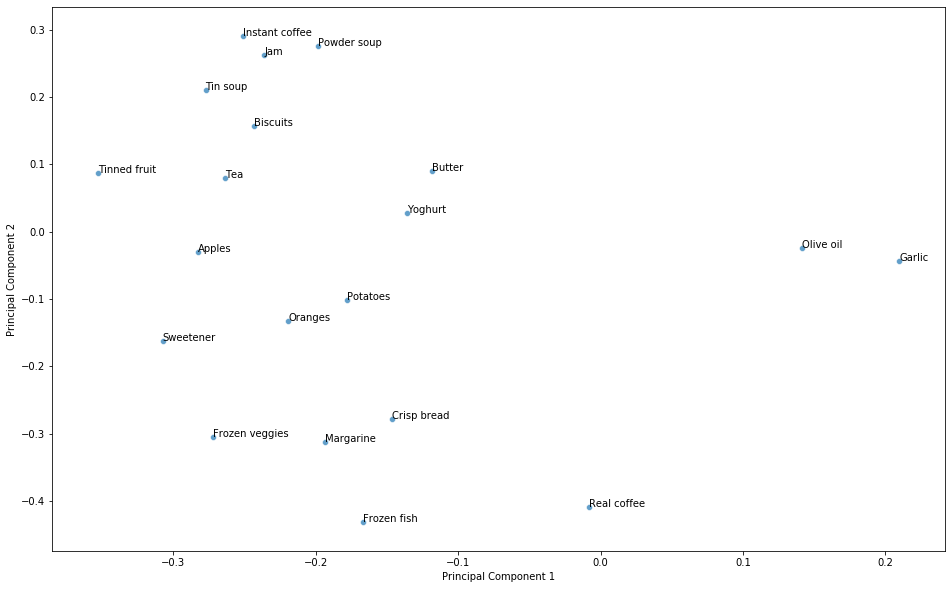
\includegraphics[height=3in]{Images/PCAFoods.png}
\caption{Food Items Plotted on Principal Components}
\end{figure}
 

\item (8 points) Now project each data point using the top two principal component vectors (thus now each data point will be represented using a two-dimensional vector). Draw a scatter plot of two-dimensional reduced representation for each country. What pattern can you observe? You may use use a package or write your own code. 
\begin{itemize}
\item Answer:\\
Figure 15 shows the projection of the countries on the 2 principal components. We can observe some patterns in this plot. For example, the Nordic countries are on the lower part of the plot, which can be attributed to their similar styles of cuisine (eg. Fish). We also notice England and Ireland to the left and upper parts of the plots, which corresponds to their high consumption of drinks such as tea and soup. On the far right, we see Italy and Portugal, both countries that have a high use of olive Oil and Garlic in their cuisine.

It can be noted that despite performing PCA, the countries are still fairly spread out. This can be attributed to the fact that 2 principal components may not be enough to perform a complete analysis. Since there are 20 food items, it is possible that we would need more principal components in order to be able to explain a higher degree of the variability in the data.
\end{itemize}



\begin{figure}
  \centering
  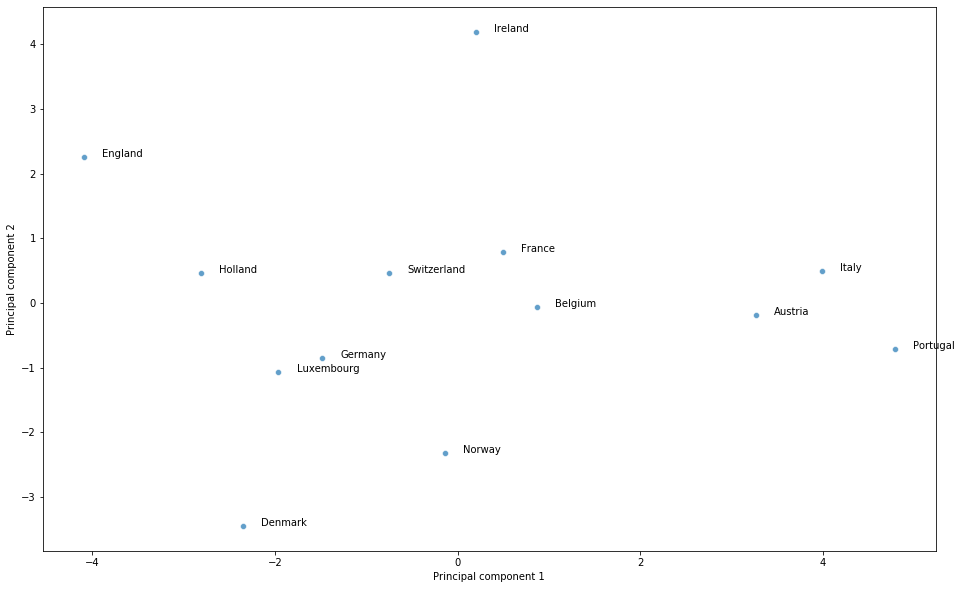
\includegraphics[height=3in]{Images/PCAScatter.png}  
\caption{Projecting Countries on the Principal Components}
\end{figure}

\end{enumerate}



\end{document}
